\documentclass[11pt]{article}
\usepackage[top=2.1cm,bottom=2cm,left=2cm,right= 2cm]{geometry}
%\geometry{landscape}                % Activate for for rotated page geometry
\usepackage[parfill]{parskip}    % Activate to begin paragraphs with an empty line rather than an indent
\usepackage{graphicx}
\usepackage{amssymb}
\usepackage{epstopdf}
\usepackage{amsmath}
\usepackage{multirow}
\usepackage{hyperref}
\usepackage{changepage}
\usepackage{lscape}
\usepackage{ulem}
\usepackage{multicol}
\usepackage{float}
\usepackage{dashrule}
\usepackage[usenames,dvipsnames]{color}
\usepackage{enumerate}
\newcommand{\urlwofont}[1]{\urlstyle{same}\url{#1}}
\newcommand{\degree}{\ensuremath{^\circ}}
\newcommand{\hl}[1]{\textbf{\underline{#1}}}



\DeclareGraphicsRule{.tif}{png}{.png}{`convert #1 `dirname #1`/`basename #1 .tif`.png}

\newenvironment{choices}{
\begin{enumerate}[(a)]
}{\end{enumerate}}

%\newcommand{\soln}[1]{\textcolor{MidnightBlue}{\textit{#1}}}	% delete #1 to get rid of solutions for handouts
\newcommand{\soln}[1]{ \vspace{1.35cm} }

%\newcommand{\solnMult}[1]{\textbf{\textcolor{MidnightBlue}{\textit{#1}}}}	% uncomment for solutions
\newcommand{\solnMult}[1]{ #1 }	% uncomment for handouts

%\newcommand{\pts}[1]{ \textbf{{\footnotesize \textcolor{black}{(#1)}}} }	% uncomment for handouts
\newcommand{\pts}[1]{ \textbf{{\footnotesize \textcolor{blue}{(#1)}}} }	% uncomment for handouts

\newcommand{\note}[1]{ \textbf{\textcolor{red}{[#1]}} }	% uncomment for handouts

\begin{document}


\enlargethispage{\baselineskip}

Fall 2019 \hfill Jingchen (Monika) Hu\\

\begin{center}
{\huge MATH 347 Homework 4 (Total 45 points)}	\\
Due: Thursday 10/31, at the beginning of class
\end{center}
\vspace{0.5cm}

\textbf{Name:} \rule{6cm}{0.5pt}\\
%\textbf{List the questions you hope be to explained in class (no more than three)} \rule{3cm}{0.5pt}	 \\


{\bf
\begin{itemize}
\item Print out this cover page and staple with your homework.
\item Show all work. Incomplete solutions will be given no credit.
\item You may prepare either hand-written or typed solutions,
but make sure that they are legible.
Answers that cannot be read will be given no credit.
\item R graphical outputs must be printed instead of hand-drawn.

\end{itemize}
}

%\underline{Textbook  Chapter 1   }

\begin{enumerate}

%%%%%%%%%%%%%%%%%%%%%%%%%%%%%%%%%%%%%%%%%%%%%%

    \item
    ({\it{12 points; 3 points each part}}) \\
Suppose two people, Chrystal and Danny, have different prior beliefs about the average number of ER visits during the 10pm - 11pm time period.  Chrystal's prior information is matched to a Gamma distribution with parameters $\alpha = 70$ and $\beta = 10$, and Danny's beliefs are matched to a Gamma distribution with $\alpha = 33.3$ and $\beta = 3.3$.

%  The two gamma priors are displayed in Figure \ref{fig:gammapriors}.
%
%\begin{figure}[h!]
%\begin{center}
%\includegraphics[scale=0.5]{figures/chapter7/gammapriors.pdf}
%\caption{\label{fig:gammapriors} Two gamma priors for the average number of visits to ER during a particular hour in the evening.}
%\end{center}
%\end{figure}

\begin{enumerate}
\item Using the \texttt{rgamma} or the \texttt{dgamma} functions to plot these two gamma priors on the same graph. (Hint: if you use \texttt{dgamma}, you can let the range of $x$ be (0, 20].)

\item Compare the priors of Chrystal and Danny with respect to average value and spread.  Which person believes that there will be more ER visits, on average?  Which person is more confident of his/her/their ``best guess" at the average number of ER visits?

\item Using the \texttt{qgamma} function, construct a 90\% credible interval for $\lambda$ using Chrystal's prior and Danny's prior.

\item After some thought, Chrystal believes that her best prior guess at $\lambda$ is correct, but she is less confident in this guess.  Explain how Chrystal can adjust the parameters of her gamma prior to reflect this new prior belief. (Hint: the mean and variance of $\textrm{Gamma}(\alpha, \beta)$ is $\frac{\alpha}{\beta}$ and $\frac{\alpha}{\beta^2}$ respectively.)

%\item Danny also revisits his prior.  His best guess at the average number of ER visits is now 3 larger than his previous best guess, but the degree of confidence in this guess hasn't changed.  Explain how Danny can adjust the parameters of his gamma prior to reflect this new prior belief.
\end{enumerate}


 \item
    ({\it{9 points; 3 points each part}}) \\
    Continuing from Question 1. A hospital collects the number of patients in the emergency room (ER) admitted between 10 pm and 11 pm for each day of a week. Table \ref{table:ERvisits} records the day and the number of ER visits for the given day.

\begin{table}[htb]
\caption{\label{table:ERvisits} Data for ER visits in a given week.}
\begin{center}
\begin{tabular}{|c|c|} \hline
Day & Number of ER visits\\ \hline
Sunday & 8 \\
Monday & 6 \\
Tuesday & 6 \\
Wednesday & 9 \\
Thursday & 8 \\
Friday & 9 \\
Saturday & 7 \\ \hline
\end{tabular}
\end{center}
\label{default}
\end{table}%

Suppose one assumes Poisson sampling for the counts, and a conjugate Gamma prior with parameters $\alpha = 70$ and $\beta = 10$ for the Poisson rate parameter $\lambda$ (i.e. Chrystal's first prior).

\begin{enumerate}

\item Given the sample shown in Table \ref{table:ERvisits}, obtain the posterior distribution for $\lambda$ through the Gamma-Poisson conjugacy. Obtain a 95\% posterior credible interval for $\lambda$. 

\item Suppose a hospital administrator states that the average number of ER visits during any evening hour does not exceed 6.  By computing a posterior probability, evaluate the validity of the administrator's statement.

\item The hospital is interested in predicting the number of ER visits between 10 pm and 11 pm for another week. Use simulations to generate posterior predictions of the number of ER visits for another week (seven days).

\end{enumerate}



 \item
    ({\it{12 points; 3 points each part}}) \\
Suppose that we want inference about an unknown number of animals $N$ in a
  fixed-size population.  On five separate days, we take
  photographs of some areas where they reside, and count the number of
  animals in the photos ($y_1, \dots, y_5$).  Suppose further than
  each animal has a constant probability $\theta$ of appearing in a
  photograph, and that appearances are independent across animals and
  days.  A reasonable model for such data is a binomial distribution, $y_i \sim
\text{Binomial}(N, \theta)$.  In our setting, neither the number of trials $N$ nor the
probability $\theta$ are known.

%\vspace{12pt}

To get a posterior distribution for $N$ and $\theta$, we propose the following system
of models (Raftery 1988)
\begin{eqnarray*}
y_i \mid N, \theta &\sim& \text{Binomial}(N, \theta) \\
N \mid \theta, \lambda &\sim& \text{Poisson}(\lambda / \theta) \\
f(\lambda , \theta) &\propto& 1 / \lambda
\end{eqnarray*}
where $\lambda > 0$ is a continuous random variable introduced to help
with computations.

\begin{enumerate}



\item Write the expression of the joint posterior distribution, $p(N,
  \theta, \lambda \mid y_1, \dots, y_5)$, up to a multiplicative
  constant.


\item Find an expression for the conditional distribution, $f(\lambda \mid y_1,
  \dots, y_5, N, \theta)$. Write the name of the distribution, and specify
expressions for its parameter values.


\item Find the kernel of the posterior distribution $f(N, \theta
  \mid y_1, \dots, y_5)$ by integrating $f(N, \theta, \lambda \mid y_1, \dots, y_5)$ with respect to
  $\lambda$.  You don't need to name it; just write its mathematical form.


\item Find the conditional distribution, $f(\theta \mid y_1,
  \dots, y_5, N)$. Write the name of the distribution, and specify
expressions for its parameter values.


\end{enumerate}



 \item
    ({\it{12 points; 3 points each part}}) \\
    Consider a three-component mixture model, where the posterior for parameter $\mu$ is:
    \begin{equation}
    \mu \mid y \sim 0.45 \times \textrm{Normal}(-3, (1/3)^2) + 0.1 \times \textrm{Normal}(0, (1/3)^2) + 0.45 \times \textrm{Normal}(3, (1/3)^2).
    \label{eq:postmu}
    \end{equation}
    How can we draw samples from this posterior? 
    
    \begin{itemize}
    \item[] {\underline{Approach 1: Monte Carlo approximation}}\\
    If we introduce a ``mixture component indicator", $\delta$, an unobserved latent variable, the sampling can be greatly simplified, as in the following:
    \begin{itemize}
    \item[-] $\delta = 1$, then $\mu \mid \delta, y \sim \textrm{Normal}(-3, (1/3)^2)$ and $p(\delta = 1 \mid y) = 0.45$.
    \item[-] $\delta = 2$, then $\mu \mid \delta, y \sim \textrm{Normal}(0, (1/3)^2)$ and $p(\delta = 2 \mid y) = 0.1$.
    \item[-] $\delta = 3$, then $\mu \mid \delta, y \sim \textrm{Normal}(3, (1/3)^2)$ and $p(\delta = 3 \mid y) = 0.45$.
    \end{itemize}
    Therefore, we can draw $\delta$ and then draw $\mu$ given $\delta$ through Monte Carlo approximation. Figure \ref{fig:MCdensity} is the histogram of $\mu$ from 1000 Monte Carlo draws with posterior density as a solid line.
    
    
        \item[] {\underline{Approach 2: Markov chain Monte Carlo - Gibbs}}\\
    We can also derive the full conditional posterior distributions for $\pi(\mu \mid \delta, y)$ and $\pi(\delta \mid \mu, y)$, and use a Gibbs sampler to sample the posterior of $\mu$. The full conditional posterior distributions are eliminated for brevity, but be convinced that a Gibbs sampler can be developed for this case. Figure \ref{fig:MCMCdensity} is the histogram of $\mu$ from 1000 MCMC/Gibbs draws with posterior density as a solid line. Note that the initial values are $\mu = -6$ and $\delta = 1$.



\begin{multicols}{2}
\begin{figure}[H]
\begin{center}
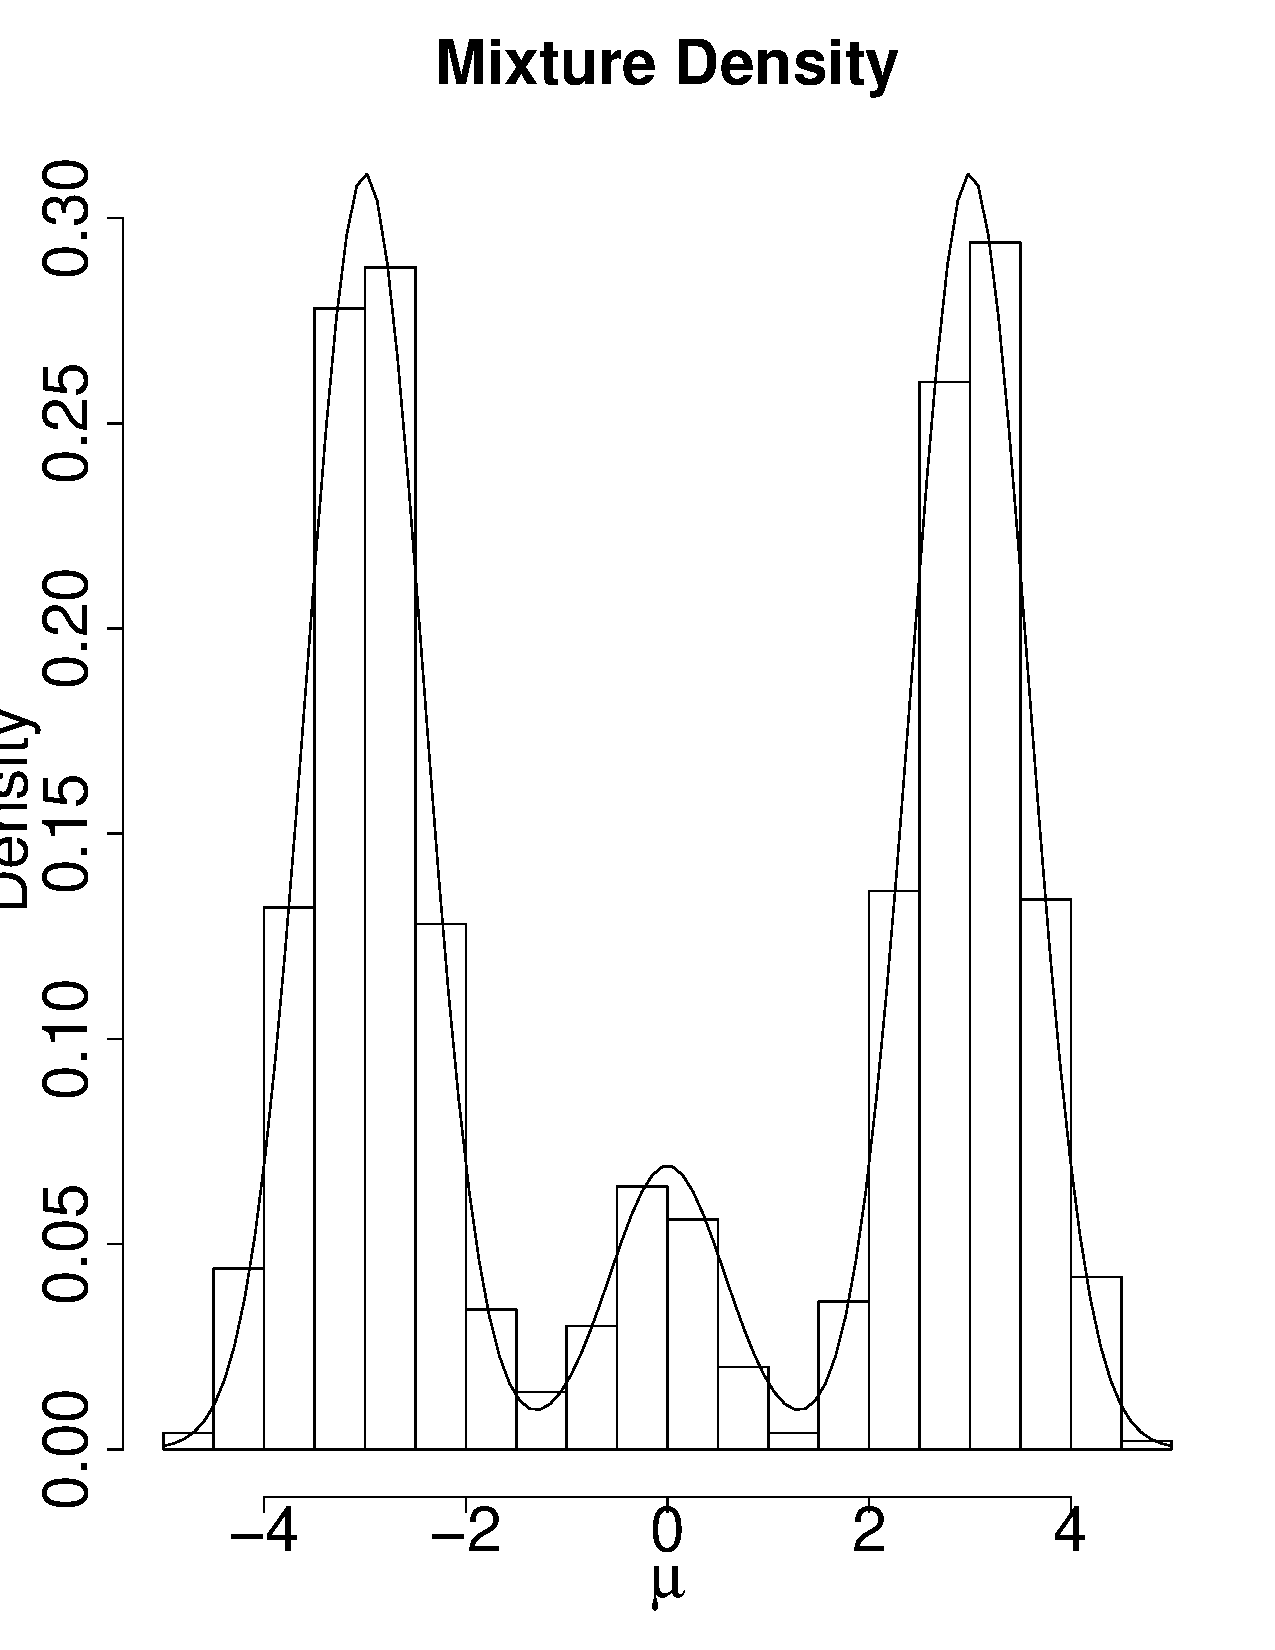
\includegraphics[scale=0.3]{figures/MCdensity}
\caption{\label{fig:MCdensity} Histogram of 1000 samples of $\mu$ from Monte Carlo approximation.}
\end{center}
\end{figure}

\begin{figure}[H]
\begin{center}
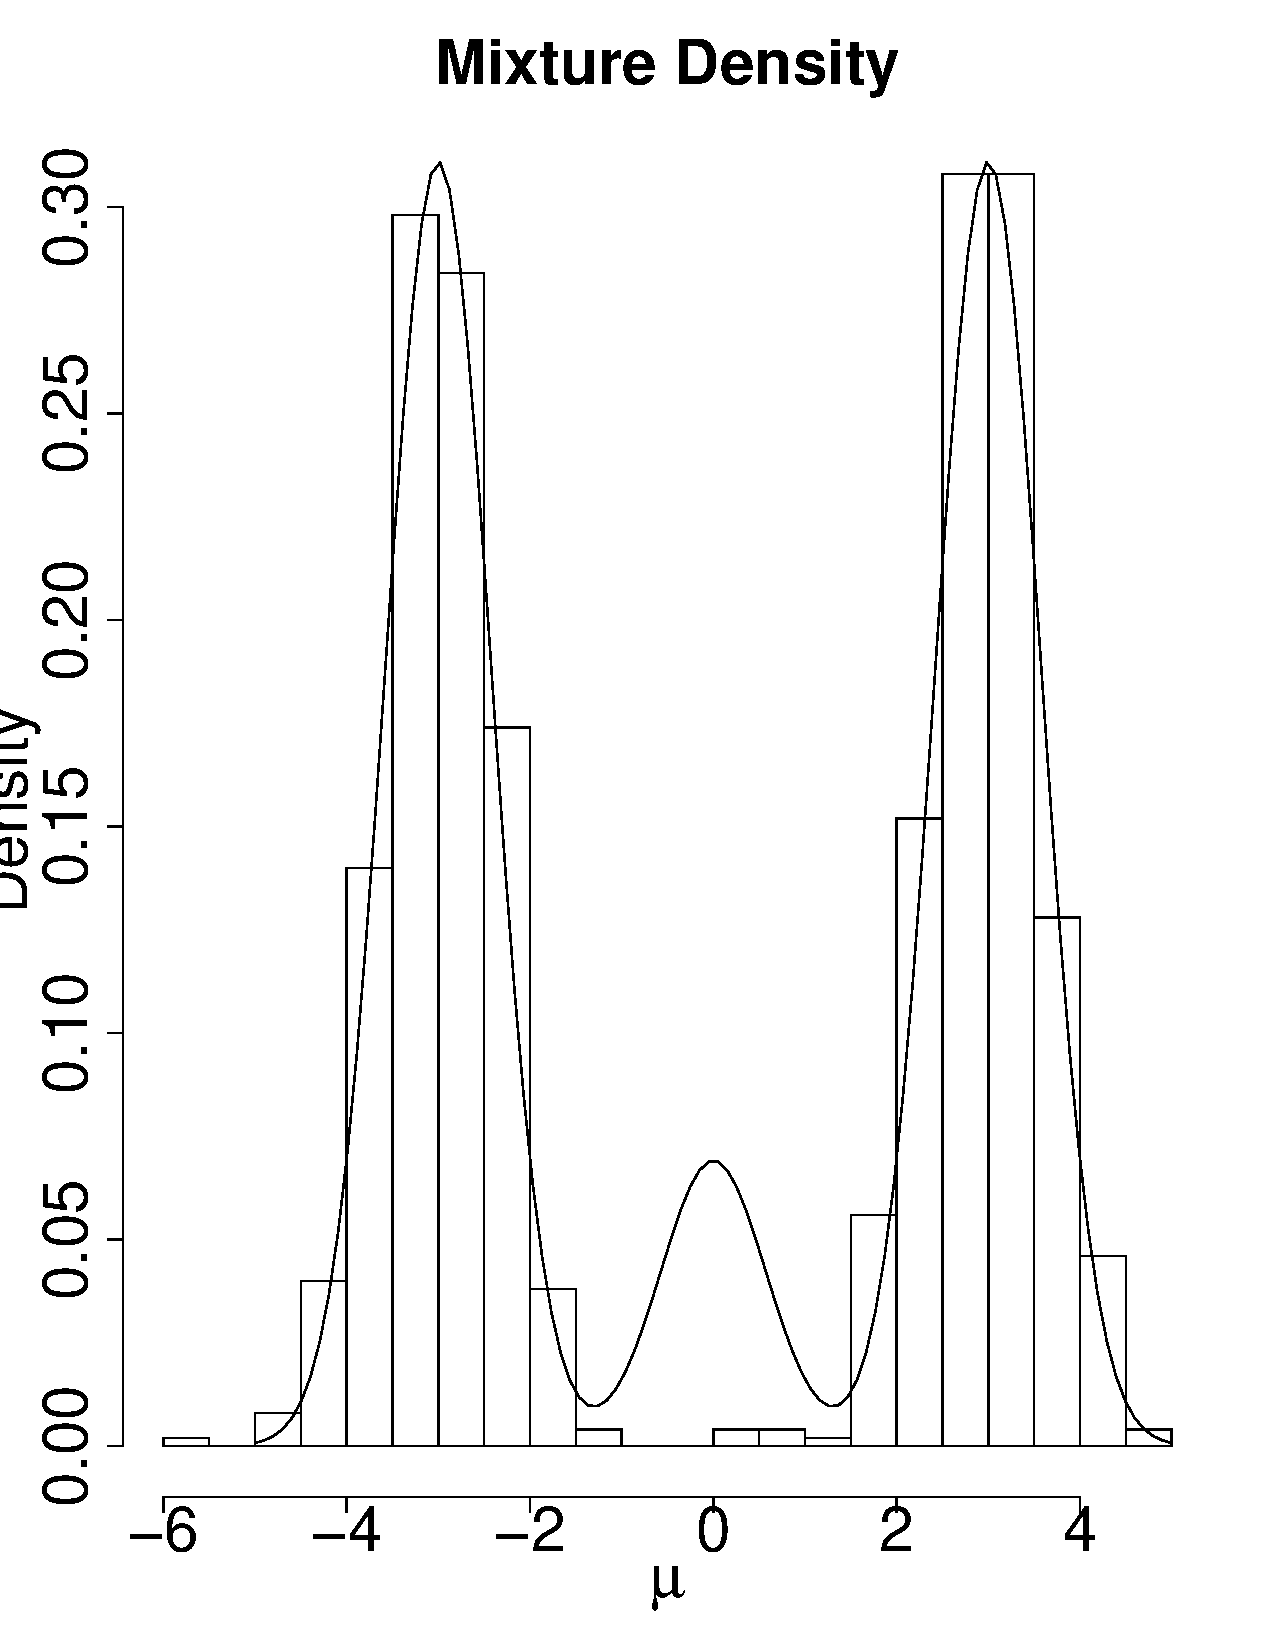
\includegraphics[scale=0.3]{figures/MCMCdensity}
\caption{\label{fig:MCMCdensity} Histogram of 1000 samples of $\mu$ from MCMC/Gibbs.}
\end{center}
\end{figure}

\end{multicols}

Sometimes, a regular scatterplot could be more descriptive of the problem. See Figure \ref{fig:MCscatter} for a scatterplot of 1000 samples of $\mu$ from Monte Carlo approximation, and Figure \ref{fig:MCMCscatter} for a scatterplot of 1000 samples of $\mu$ from MCMC/Gibbs. Think carefully with respect to the posterior density in Equation (\ref{eq:postmu}).

\newpage
\begin{multicols}{2}
\begin{figure}[H]
\begin{center}
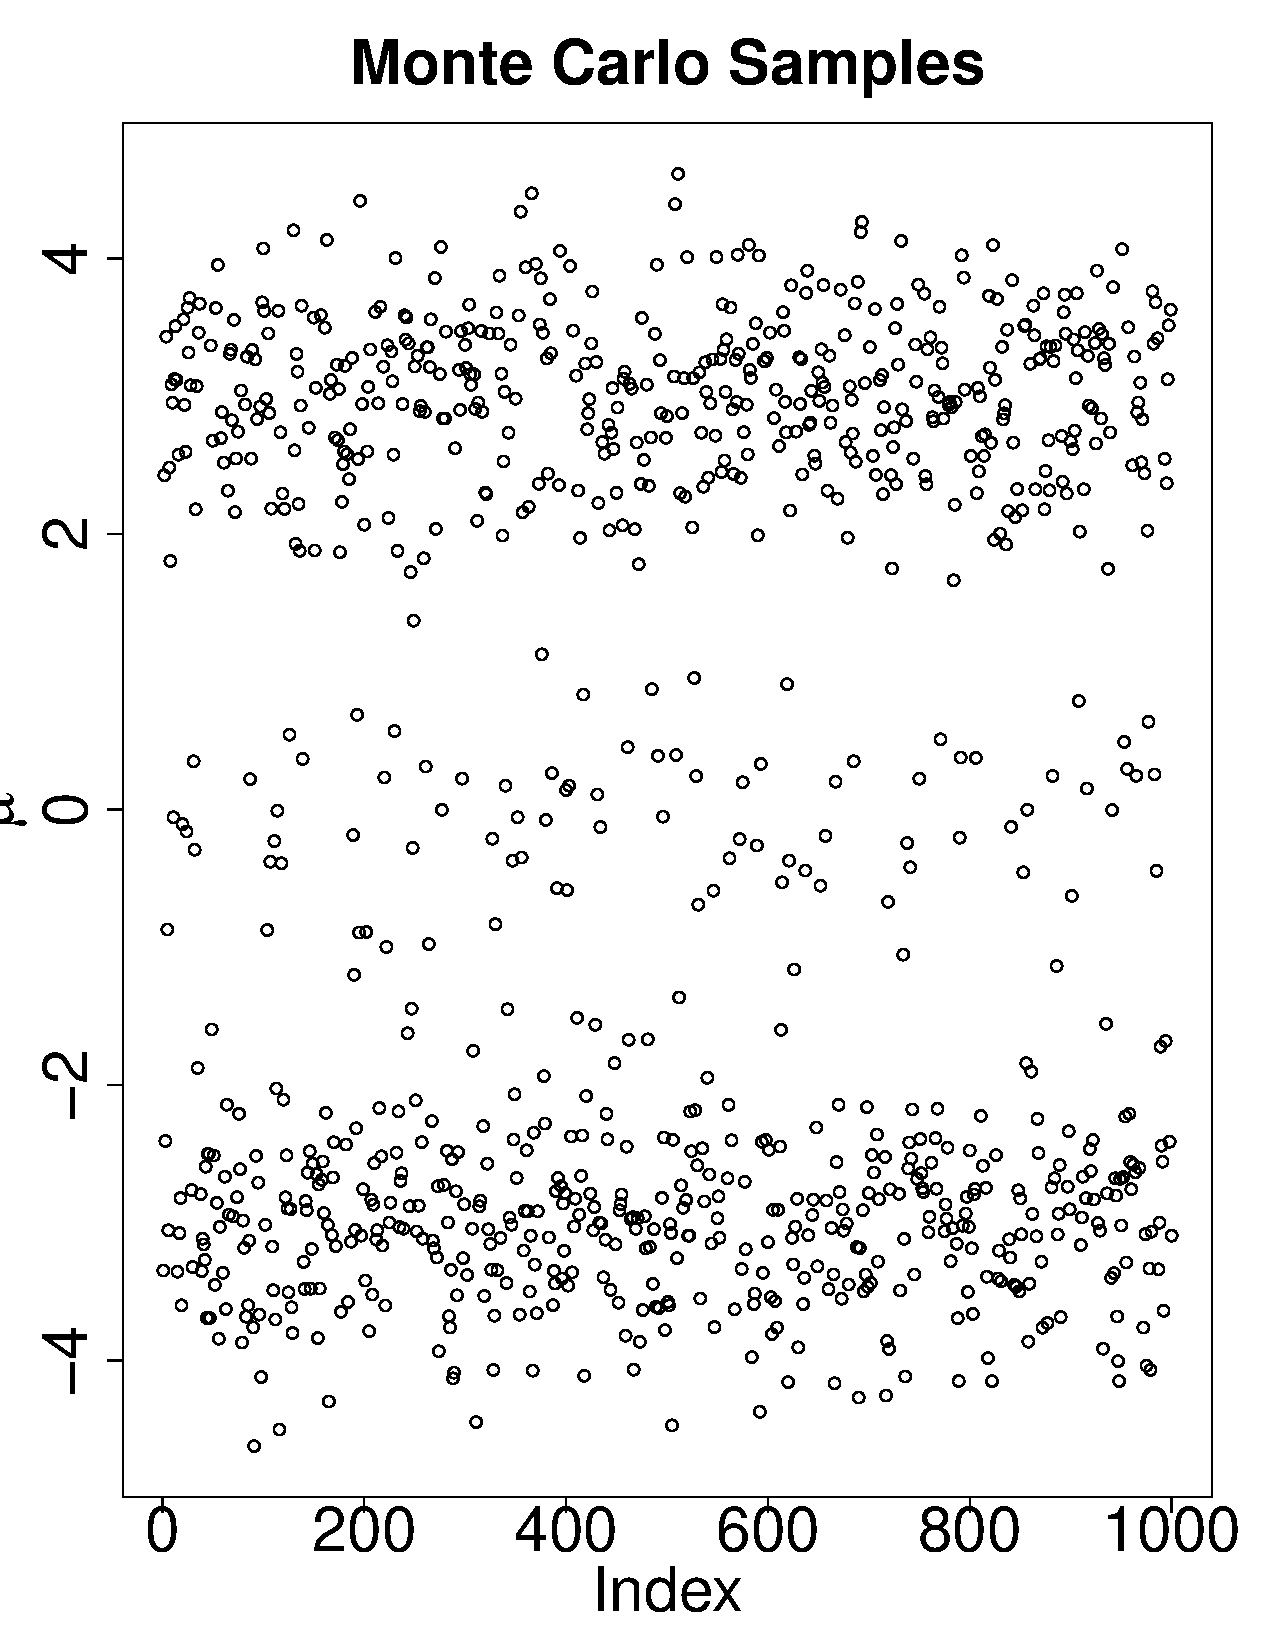
\includegraphics[scale=0.3]{figures/MCscatter}
\caption{\label{fig:MCscatter}1000 samples of $\mu$ from Monte Carlo approximation.}
\end{center}
\end{figure}

\begin{figure}[H]
\begin{center}
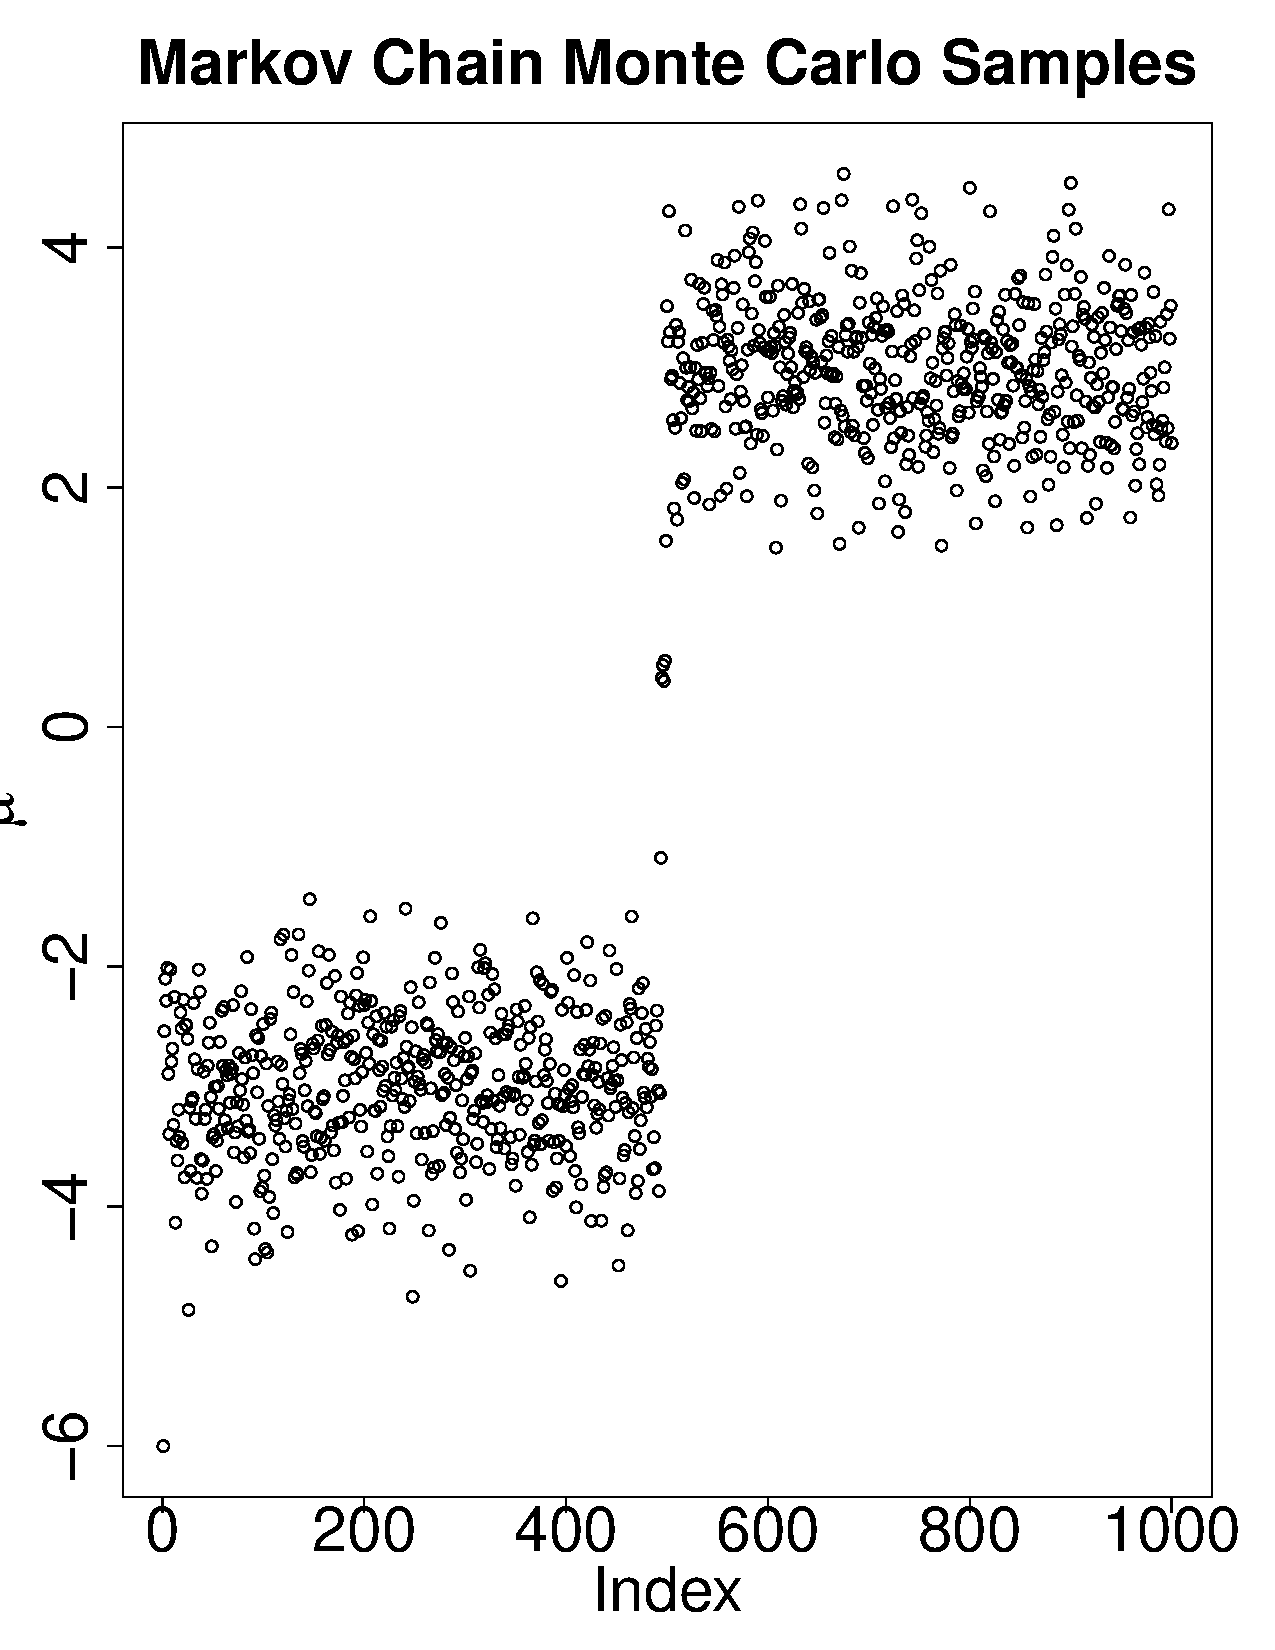
\includegraphics[scale=0.3]{figures/MCMCscatter}
\caption{\label{fig:MCMCscatter} 1000 samples of $\mu$ from MCMC/Gibbs.}
\end{center}
\end{figure}

\end{multicols}


\end{itemize}

\begin{enumerate}

\item Compare Figure \ref{fig:MCdensity} with Figure \ref{fig:MCMCdensity}, and Figure \ref{fig:MCscatter} with Figure \ref{fig:MCMCscatter}. What problems do you expect to show up when you perform MCMC diagnostics for $\mu$?

\item Examine the traceplots of $\mu$ from Monte Carlo approximation in Figure \ref{fig:MCtrace} and of $\mu$ from MCMC/Gibbs in Figure \ref{fig:MCMCtrace}. What is the issue with MCMC/Gibbs mixing?

\item Examine the ACF plots of $\mu$ from Monte Carlo approximation in Figure \ref{fig:MCacf} and of $\mu$ from MCMC in Figure \ref{fig:MCMCacf}. Also, the effective sample size of MC and MCMC/Gibbs are 1000 and 1.70 respectively. What is the issue with MCMC/Gibbs mixing?

\item Describe what you would do to improve the MCMC/Gibbs mixing.

\newpage
\begin{multicols}{2}
\begin{figure}[H]
\begin{center}
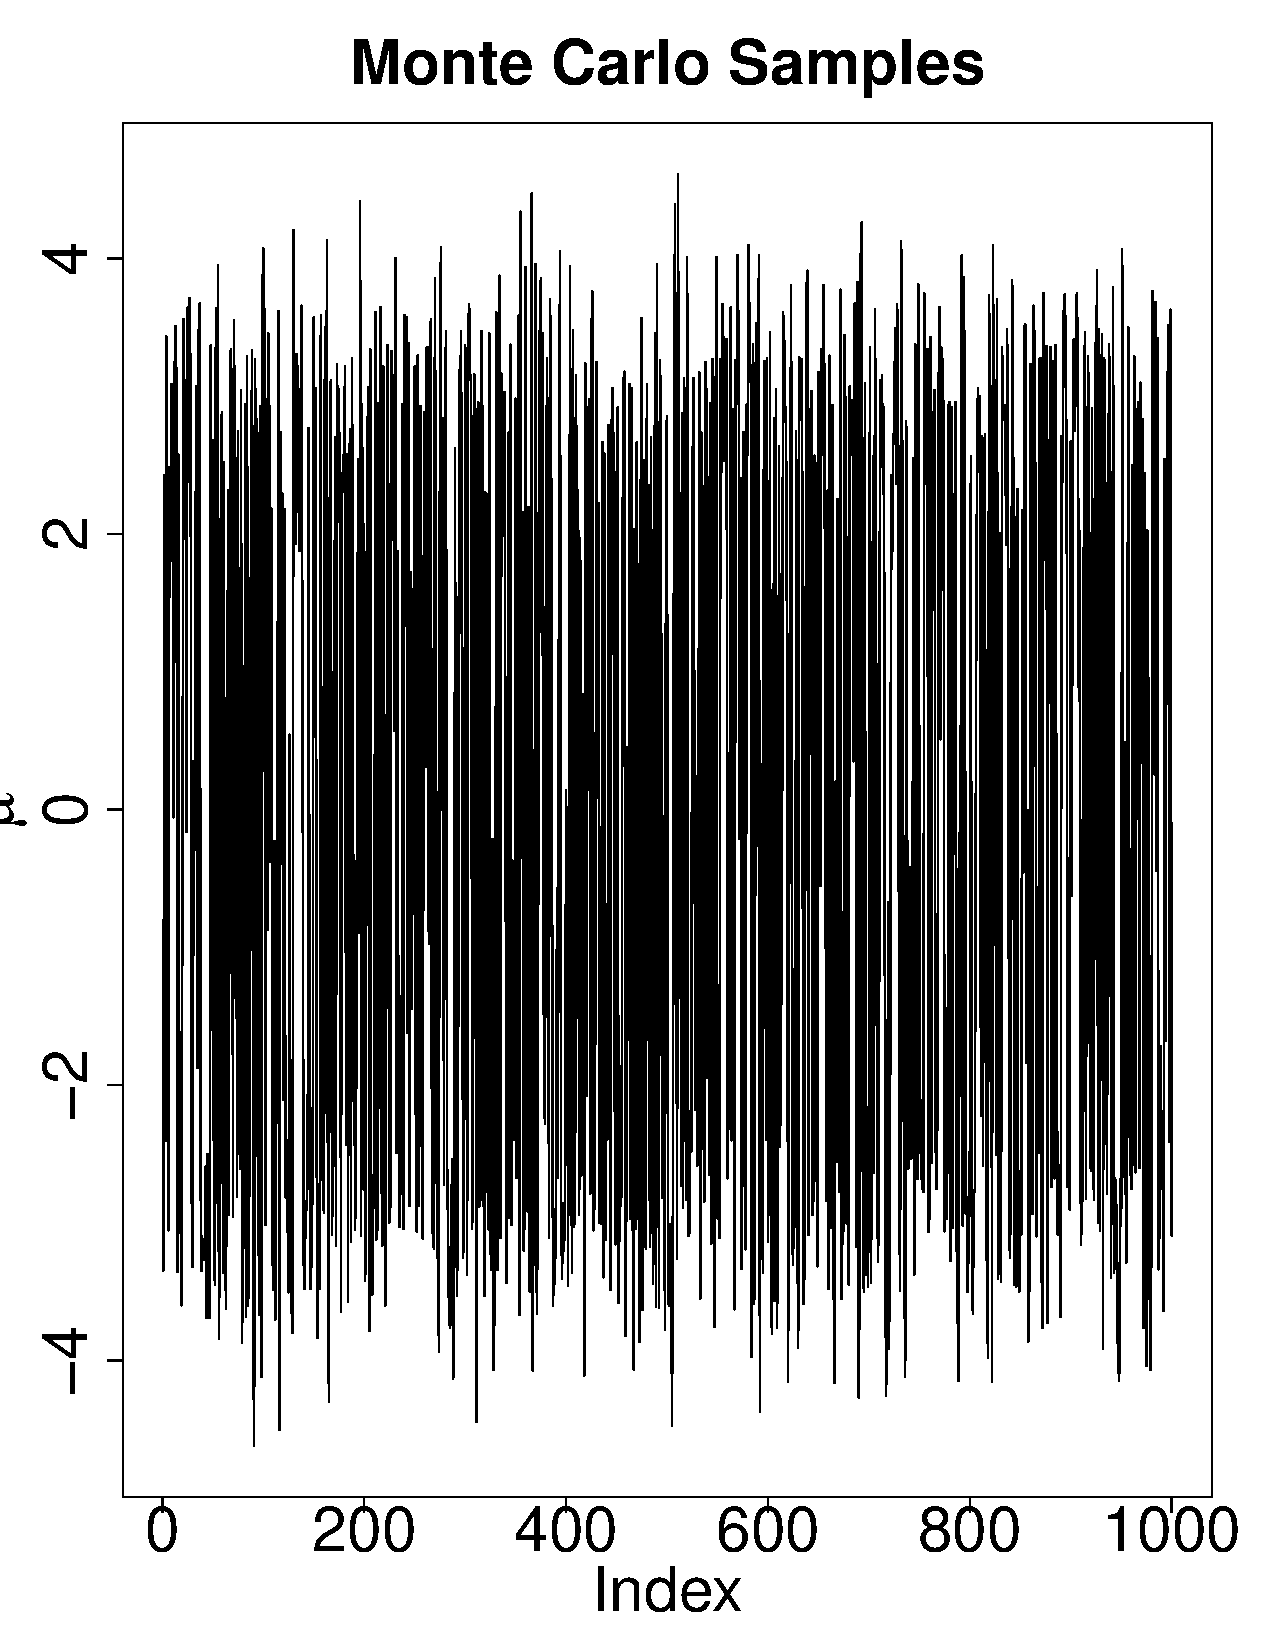
\includegraphics[scale=0.3]{figures/MCtrace}
\caption{\label{fig:MCtrace} Traceplot of $\mu$ from Monte Carlo approximation.}
\end{center}
\end{figure}

\begin{figure}[H]
\begin{center}
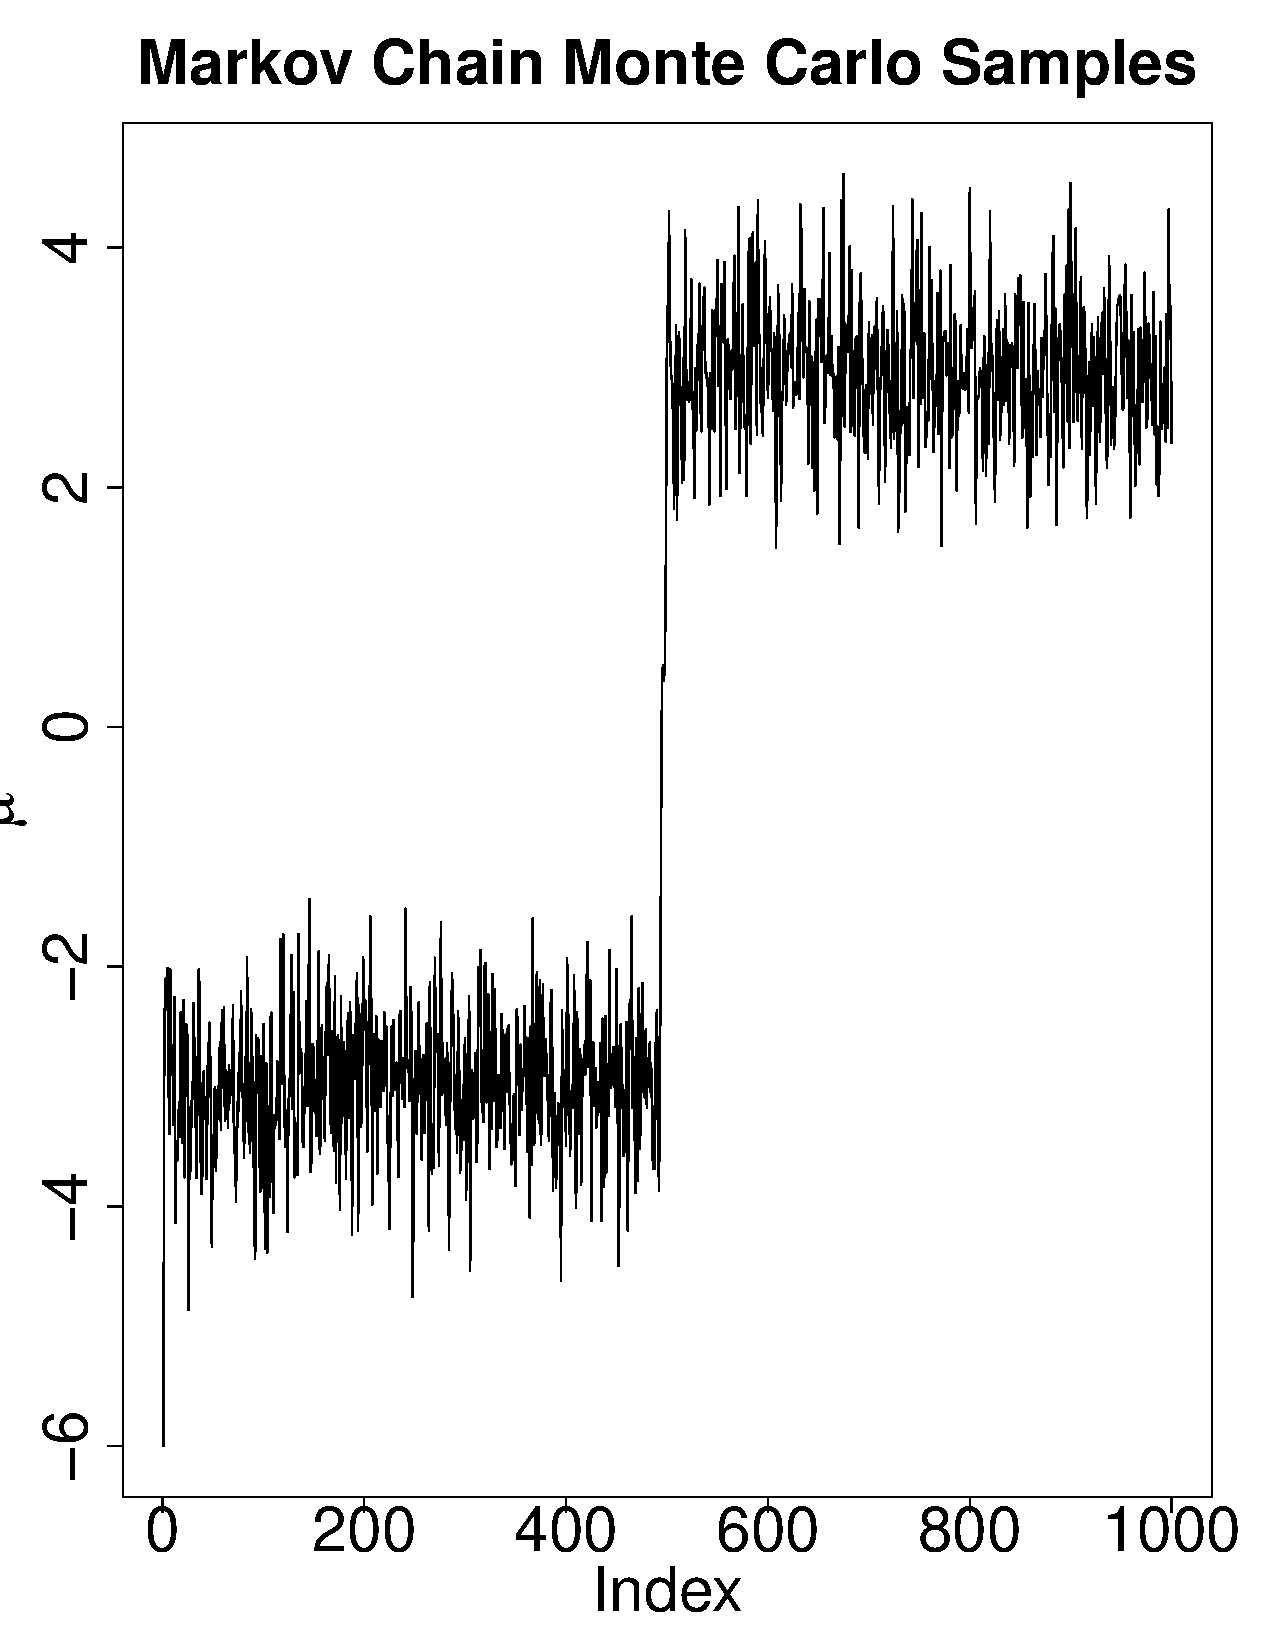
\includegraphics[scale=0.3]{figures/MCMCtrace}
\caption{\label{fig:MCMCtrace} Traceplot of of $\mu$ from MCMC/Gibbs.}
\end{center}
\end{figure}

\end{multicols}



\begin{multicols}{2}
\begin{figure}[H]
\begin{center}
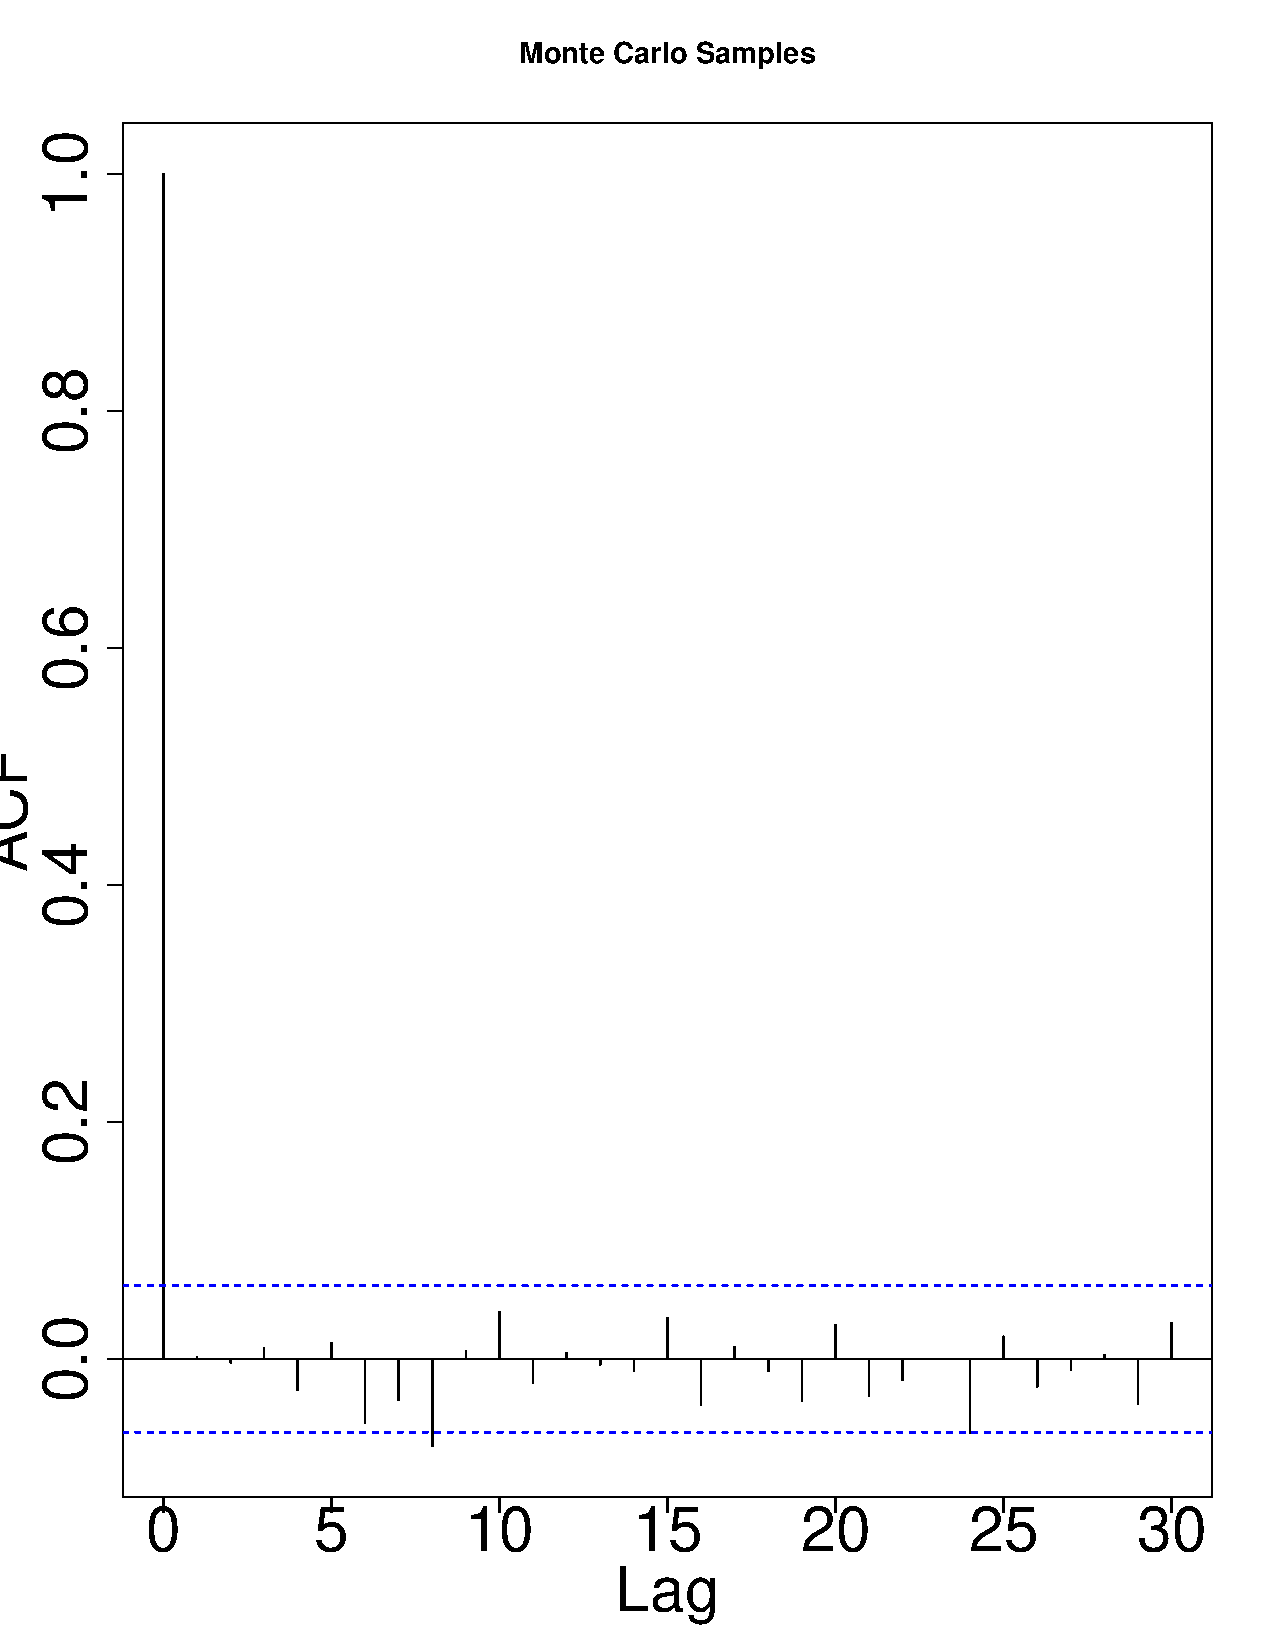
\includegraphics[scale=0.3]{figures/MCacf}
\caption{\label{fig:MCacf} ACF plot of $\mu$ from Monte Carlo approximation.}
\end{center}
\end{figure}

\begin{figure}[H]
\begin{center}
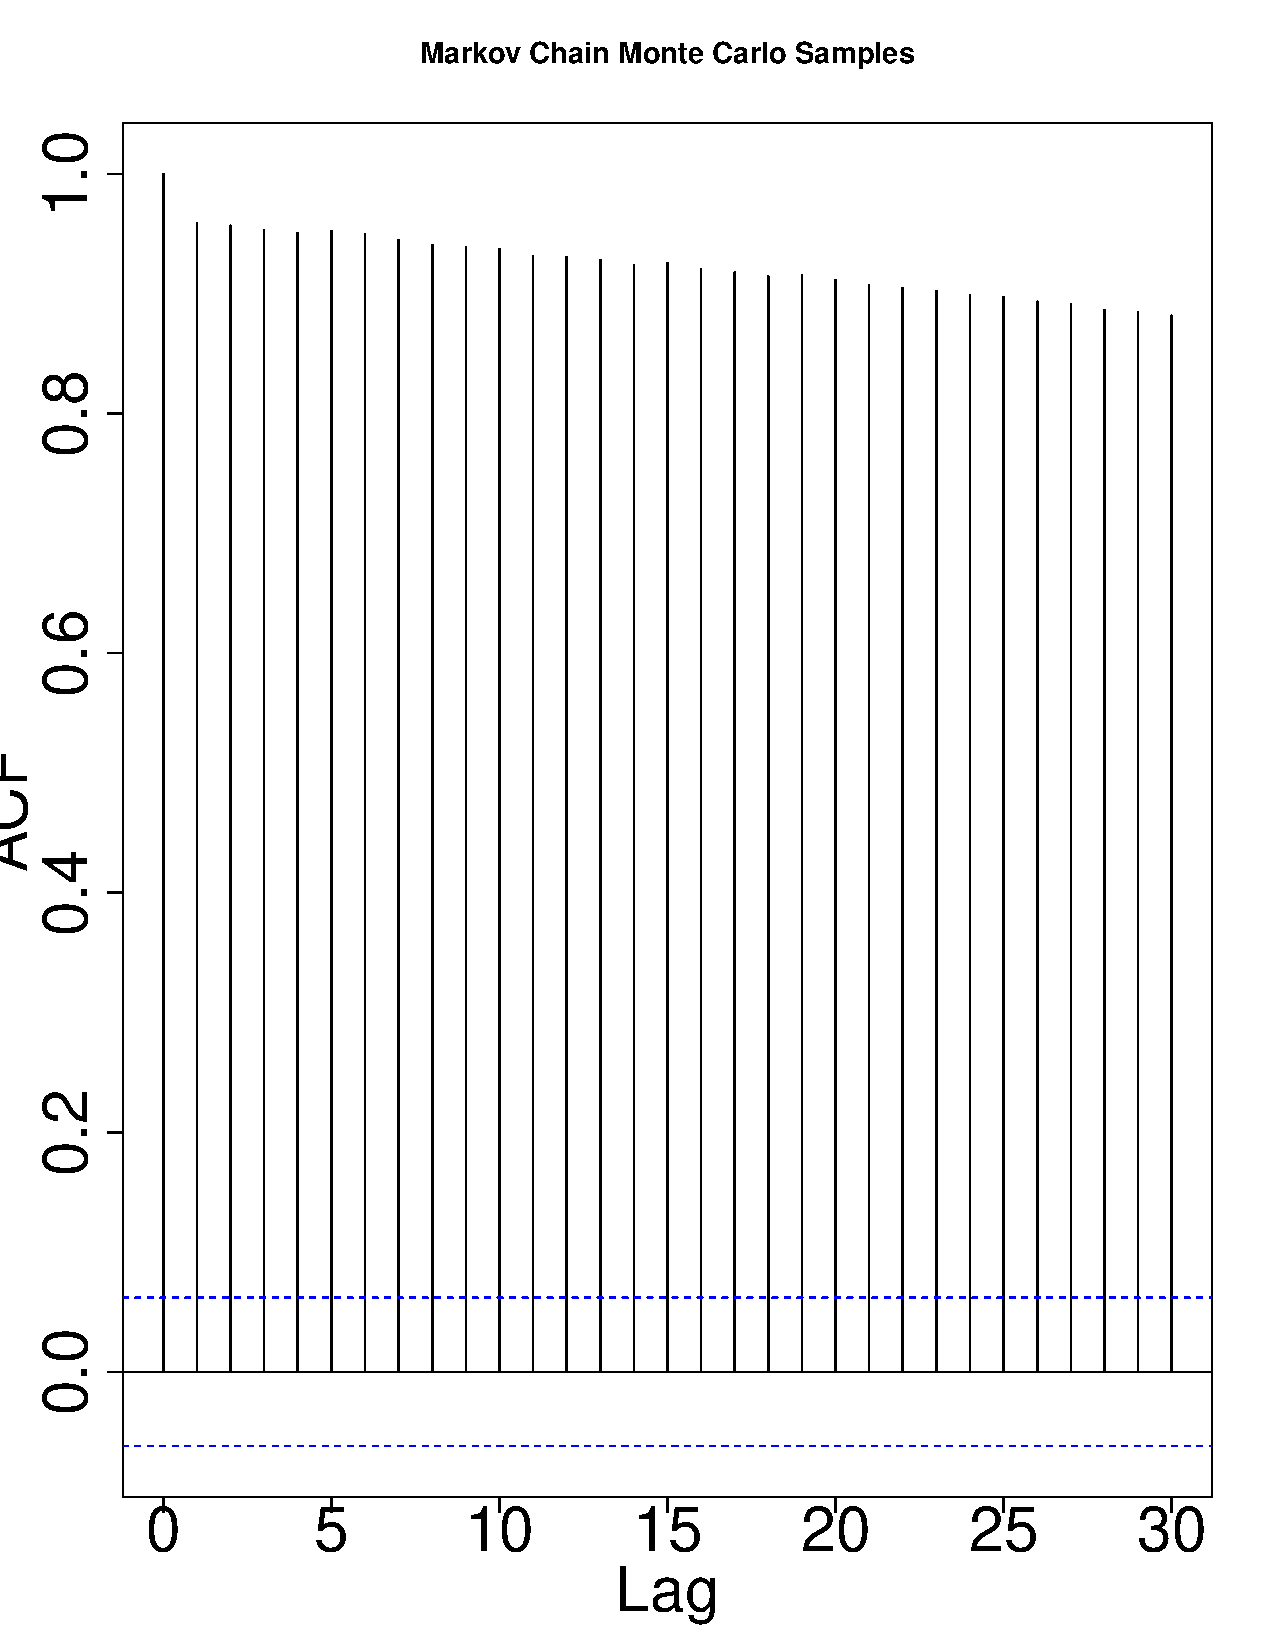
\includegraphics[scale=0.3]{figures/MCMCacf}
\caption{\label{fig:MCMCacf} ACF plot of of $\mu$ from MCMC/Gibbs.}
\end{center}
\end{figure}

\end{multicols}


\end{enumerate}


\end{enumerate}









\end{document} 